%iffalse
\let\negmedspace\undefined
\let\negthickspace\undefined
\documentclass[journal,12pt,onecolumn]{IEEEtran}
\usepackage{cite}
\usepackage{amsmath,amssymb,amsfonts,amsthm}
\usepackage{algorithmic}
\usepackage{graphicx}
\usepackage{textcomp}
\usepackage{xcolor}
\usepackage{txfonts}
\usepackage{listings}
\usepackage{enumitem}
\usepackage{mathtools}
\usepackage{gensymb}
\usepackage{comment}
\usepackage[breaklinks=true]{hyperref}
\usepackage{tkz-euclide} 
\usepackage{listings}
\usepackage{gvv}
\def\inputGnumericTable{}                                 
\usepackage[latin1]{inputenc}                              
\usepackage{color}                                         
\usepackage{array}                                        
\usepackage{longtable}                                     
\usepackage{calc}                                          
\usepackage{multirow}                                      
\usepackage{hhline}                                        
\usepackage{ifthen}                                        
\usepackage{lscape}
\newtheorem{theorem}{Theorem}[section]
\newtheorem{problem}{Problem}
\newtheorem{proposition}{Proposition}[section]
\newtheorem{lemma}{Lemma}[section]
\newtheorem{corollary}[theorem]{Corollary}
\newtheorem{example}{Example}[section]
\newtheorem{definition}[problem]{Definition}
\newcommand{\BEQA}{\begin{eqnarray}}
\newcommand{\EEQA}{\end{eqnarray}}
\newcommand{\define}{\stackrel{\triangle}{=}}
\theoremstyle{remark}
\newtheorem{rem}{Remark}
\graphicspath{ {./Figures/} }
\usepackage{float} % For the [H] float option
\usepackage{textcomp}
\usepackage{multicol}
\begin{document}

     \Large\textbf{Q.1 -- Q.20 carry one mark each.} \\[10mm]


\begin{enumerate}[start=1, label=Q.\arabic*]
    \item The number of chords in the graph of the given circuit will be
\begin{figure}[H]
    \centering
    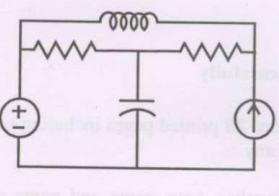
\includegraphics[width=\columnwidth]{Fig/q1.png}
    \caption{}
\end{figure}


\begin{enumerate}
\begin{multicols}{4}
\item 3
\item 4
\item 5
\item 6
\end{multicols}
\end{enumerate}
\hfill (GATE EE 2008)




\item The Thevenin's equivalent of a circuit operating at $\omega=5rad/s$ has $V_{oc}=3.17 \angle - 15.9 \degree V$ and $Z_o = 2.38 - j0.667\omega$ . At this frequency, the minimal
realization of the Thevenin's impedance will have a

\begin{multicols}{2}
\begin{enumerate}

\item resistor and a capacitor and an inductor
\item resistor and a capacitor
\item resistor and an inductor
\item capacitor and an inductor
\end{enumerate}
\end{multicols}
\hfill (GATE EE 2008)





\item A signal $e^{-\alpha t} \sin(\omega t)$ is the input to a real Linear Time Invariant system. 
Given $K$ and $\phi$ are constants, the output of the system will be of the form 
$K e^{-\beta t} \sin(\nu t + \phi)$ where
\begin{enumerate}
\item $\beta$ need not be equal to $\alpha$ but $\nu$ equal to $\omega$
    \item $\nu$ need not be equal to $\omega$ but $\beta$ equal to $\alpha$
    \item $\beta$ equal to $\alpha$ and $\nu$ equal to $\omega$
    \item $\beta$ need not be equal to $\alpha$ and $\nu$ need not be equal to $\omega$
\end{enumerate}
\hfill (GATE EE 2008)




\item X is a uniformly distributed random variable that takes values between $0$ and $1$. 
The value of $E\{X^3\}$ will be %\{ ... \} produces curly braces {}
\begin{enumerate}
\begin{multicols}{4}

    \item 0
    \item $\frac{1}{8}$
    \item $\frac{1}{4}$
    \item $\frac{1}{2}$
\end{multicols}
\end{enumerate}
\hfill (GATE EE 2008)




\item The characteristic equation of a $(3 \times 3)$ matrix $\mathbf{P}$ is defined as
\[
\alpha(\lambda) = \lvert \lambda \mathbf{I} - \mathbf{P} \rvert 
= \lambda^3 + \lambda^2 + 2\lambda + 1 = 0.
\] % /lvert is mod
If $\mathbf{I}$ denotes the identity matrix, then the inverse of matrix $\mathbf{P}$ will be

\begin{enumerate}
\begin{multicols}{4}
    \item $(\mathbf{P}^2 + \mathbf{P} + 2\mathbf{I})$
    \item $(\mathbf{P}^2 + \mathbf{P} + \mathbf{I})$
    \item $-(\mathbf{P}^2 + \mathbf{P} + \mathbf{I})$
    \item $-(\mathbf{P}^2 + \mathbf{P} + 2\mathbf{I})$
\end{multicols}
\end{enumerate}
\hfill (GATE EE 2008)




\item If the rank of a $(5 \times 6)$ matrix $\mathbf{Q}$ is $4$, then which one of the following statements is correct?

\begin{enumerate}
    \item $\mathbf{Q}$ will have four linearly independent rows and four linearly independent columns
    \item $\mathbf{Q}$ will have four linearly independent rows and five linearly independent columns
    \item $\mathbf{Q} \mathbf{Q}^T$ will be invertible
    \item $\mathbf{Q}^T \mathbf{Q}$ will be invertible
\end{enumerate}
\hfill (GATE EE 2008)




\item A function $y(t)$ satisfies the following differential equation:
\[
\frac{dy(t)}{dt} + y(t) = \delta(t)
\]
where $\delta(t)$ is the delta function. Assuming zero initial condition, and denoting the unit step function by $u(t)$, $y(t)$ can be of the form

\begin{enumerate}
    \item $e^{t}$
    \item $e^{-t}$
    \item $e^{t}u(t)$
    \item $e^{-t}u(t)$
\end{enumerate}
\hfill (GATE EE 2008)





\item The equivalent circuits of a diode, during forward biased and reverse biased
conditions, are shown in the figure
\begin{figure}[H]
    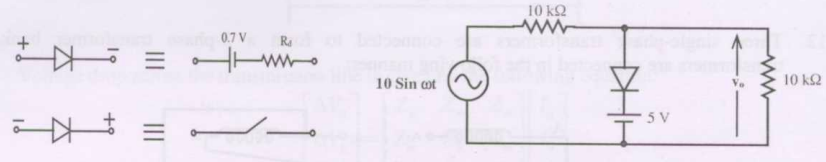
\includegraphics[width=\columnwidth]{Fig/q8.png}
    \caption{}
\end{figure}
If such a diode is used in clipper circuit of figure given above, the output voltage $(v_0)$ of the circuit will be
\begin{enumerate}
\item 
\begin{figure}[H]
    
    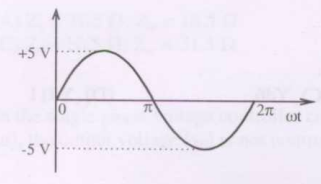
\includegraphics[width=\columnwidth]{Fig/q8A.png}
    \caption{}
\end{figure}
\item 
\begin{figure}[H]
    
    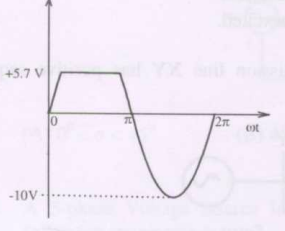
\includegraphics[width=\columnwidth]{Fig/q8C.png}
    \caption{}
\end{figure}
\item 
\begin{figure}[H]
    
    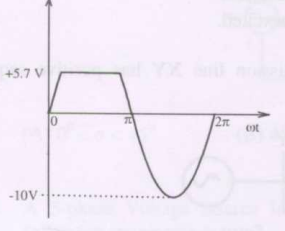
\includegraphics[width=\columnwidth]{Fig/q8C.png}
    \caption{}
\end{figure}
\item 
\begin{figure}[H]
    
    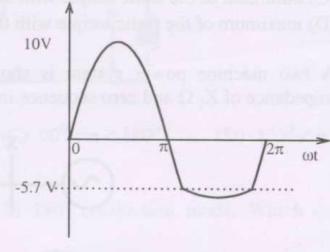
\includegraphics[width=\columnwidth]{Fig/q8D.png}
    \caption{}
\end{figure}

\end{enumerate}
\hfill (GATE EE 2008)





\item Two 8-bit ADCs, one of single slope integrating type and other of successive approximation type, 
take $T_A$ and $T_B$ times to convert $5 \ \mathrm{V}$ analog input signal to equivalent digital output. 
If the input analog signal is reduced to $2.5 \ \mathrm{V}$, the approximate time taken by the two ADCs will respectively, be

\begin{enumerate}
\begin{multicols}{4}
    
    \item $T_A, \ T_B$
    \item $\frac{T_A}{2}, \ T_B$
    \item $T_A, \ \frac{T_B}{2}$
    \item $\frac{T_A}{2}, \ \frac{T_B}{2}$
 \end{multicols}
\end{enumerate}
\hfill (GATE EE 2008)





\item An input device is interfaced with Intel 8085A microprocessor as memory mapped I/O. 
The address of the device is {2500H}. In order to input data from the device to accumulator, 
the sequence of instructions will be

\begin{enumerate}
\begin{multicols}{2}
    
    \item {LXI H, 2500H} \\
          {MOV A, M}
    \item {LXI H, 2500H} \\
          {MOV M, A}
    \item {LHLD 2500H} \\
          {MOV A, M}
    \item {LHLD 2500H} \\
          {MOV M, A}
\end{multicols}
\end{enumerate}
\hfill (GATE EE 2008)



\item Distributed winding and short chording employed in AC machines will result in

\begin{enumerate}
    \item increase in emf and reduction in harmonics.
    \item reduction in emf and increase in harmonics.
    \item increase in both emf and harmonics.
    \item reduction in both emf and harmonics.
\end{enumerate}
\hfill (GATE EE 2008)



\item Three single-phase transformers are connected to form a 3-phase transformer bank. 
The transformers are connected in the following manner: 
\begin{figure}[H]
    \centering
    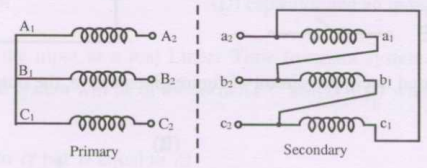
\includegraphics[width=\columnwidth]{Fig/q12.png}
    \caption{}
\end{figure}

The transformer connection will be represented by

\begin{enumerate}
\begin{multicols}{4}
    \item \(Yd0\)
    \item \(Yd1\)
    \item \(Yd6\)
    \item \(Yd11\)
    \end{multicols}
\hfill (GATE EE 2008)
\end{enumerate}



\item In a stepper motor, the detent torque means
\begin{enumerate}
    \item minimum of the static torque with the phase winding excited.
    \item maximum of the static torque with the phase winding excited.
    \item minimum of the static torque with the phase winding unexcited.
    \item maximum of the static torque with the phase winding unexcited.
\end{enumerate}
\hfill (GATE EE 2008)



\item A two machine power system is shown below. Transmission line XY has positive sequence
impedance of $Z_1 \Omega.$ and zero sequence impedance of $Z_0 \Omega.$ 

\begin{figure}[H]
    \centering
    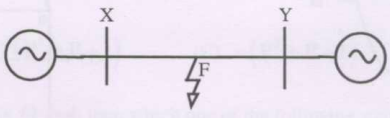
\includegraphics[width=\columnwidth]{Fig/q14.png}
    \caption{}
\end{figure}

An 'a' phase to ground fault with zero fault impedance occurs at the centre of the transmission line.
Bus voltage at X and line current from X to F for the phase 'a', are given by V Volts and
Amperes, respectively. Then, the impedance measured by the ground distance relay located at the
terminal X of line XY will be given by

\begin{enumerate}
\begin{multicols}{4}
    \item $Z_1/2 \Omega$
    \item $Z_0/2 \Omega$
    \item $Z_1+Z_0/2 \Omega$
    \item $V_0/I_0 $
    \end{multicols}
\end{enumerate}
\hfill (GATE EE 2008)


\item An extra high voltage transmission line of length $300$ km can be approximated by a lossless line having propagation constant $\beta = 0.00127$ radians per km. Then the percentage ratio of line length to wavelength will be given by

\begin{multicols}{4}
    \begin{enumerate}
        \item $24.24 \%$
        \item $12.12 \%$
        \item $19.05 \%$
        \item $6.06 \%$
    \end{enumerate}
\end{multicols}
\hfill (GATE EE 2008)


 \item  A 3-phase transmission line is shown in the figure:
 \begin{figure}[H]
     \centering
     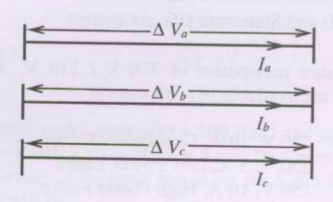
\includegraphics[width=\columnwidth]{Fig/q16-1.png}
     \caption{}
 \end{figure}
Voltage drop across the transmission line is given by the following equation:
\begin{figure}[H]
     \centering
     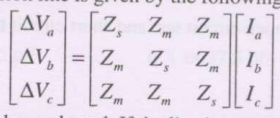
\includegraphics[width=\columnwidth]{Fig/q16-2.png}
     \caption{}
 \end{figure}

Shunt capacitance of the line can be neglected. If the line has positive sequence impedance of 15
and zero sequence impedance of 48 2, then the values of $Z_s$ and $Z_n$ will be
\begin{multicols}{2}
    \begin{enumerate}
        \item $Z_{s} = 31.5\, \Omega; Z_{m} = 16.5\, \Omega$
        \item $Z_{s} = 26\, \Omega; Z_{m} = 11\, \Omega$
        \item $Z_{s} = 16.5\, \Omega; Z_{m} = 31.5\, \Omega$
        \item $Z_{s} = 11\, \Omega; Z_{m} = 26\, \Omega$
    \end{enumerate}
\end{multicols}
\hfill (GATE EE 2008)


\item In the single phase voltage controller circuit shown in the figure, for what range of triggering angle $(\alpha)$, the output voltage $(v_{o})$ is not controllable?

\begin{figure}[H]
    \centering
    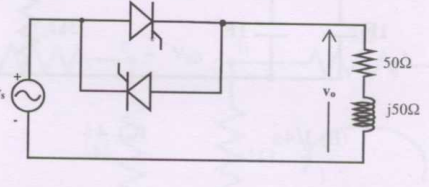
\includegraphics[width=\columnwidth]{Fig/q17.png}
    \caption{}
\end{figure}

\begin{multicols}{2}
    \begin{enumerate}
        \item $0\degree < \alpha < 45\degree$
        \item $45\degree < \alpha < 135\degree$
        \item $90\degree< \alpha < 180\degree$
        \item $135\degree < \alpha < 180\degree$
    \end{enumerate}
\end{multicols}
\hfill (GATE EE 2008)



\item A 3-phase Voltage Source Inverter is operated in \degree{180} conduction mode. Which one of the following statements is true?

\begin{enumerate}
    \item Both pole-voltage and line-voltage will have $3^{\text{rd}}$ harmonic components
    \item Pole-voltage will have $3^{\text{rd}}$ harmonic component but line-voltage will be free from $3^{\text{rd}}$ harmonic
    \item Line-voltage will have $3^{\text{rd}}$ harmonic component but pole-voltage will be free from $3^{\text{rd}}$ harmonic
    \item Both pole-voltage and line-voltage will be free from $3^{\text{rd}}$ harmonic components
\end{enumerate}
\hfill (GATE EE 2008)


\item The impulse response of a causal linear time-invariant system is given as $h(t)$. Now consider the following two statements: \\
Statement (I): Principle of superposition holds \\
Statement (II): $h(t) = 0$ for $t < 0$. \\
\\
Which one of the following statements is correct?

\begin{enumerate}
    \item Statement (I) is correct and Statement (II) is wrong
    \item Statement (II) is correct and Statement (I) is wrong
    \item Both Statement (I) and Statement (II) are wrong
    \item Both Statement (I) and Statement (II) are correct
\end{enumerate}
\hfill (GATE EE 2008)



\item It is desired to measure parameters of $230$ V / $115$ V, $2$ kVA, single-phase transformer. The following wattmeters are available in a laboratory: \\
\\
$W_1$: $250$ V, $10$ A, Low Power Factor \\
$W_2$: $250$ V, $5$ A, Low Power Factor \\
$W_3$: $150$ V, $10$ A, High Power Factor \\
$W_4$: $150$ V, $5$ A, High Power Factor \\
\\
The wattmeters used in open circuit test and short circuit test of the transformer will respectively be

\begin{enumerate}
    \item $W_1$ and $W_2$
    \item $W_2$ and $W_4$
    \item $W_1$ and $W_4$
    \item $W_2$ and $W_3$
\end{enumerate}
\hfill (GATE EE 2008)


\Large\textbf{Q.21 -- Q.75 carry one mark each.} \\[10mm]

\item The time constant for the given circuit will be

\begin{figure}[H]
    \centering
    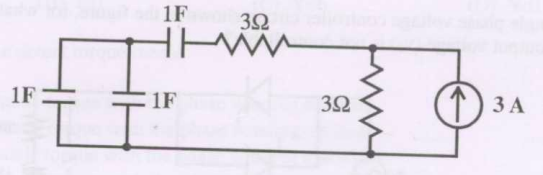
\includegraphics[width=\columnwidth]{Fig/q21.png}
    \caption{}
\end{figure}

\begin{multicols}{4}
\begin{enumerate}
    \item $1/9$ s
    \item $1/4$ s
    \item $4$ s
    \item $9$ s
\end{enumerate}
\end{multicols}
\hfill (GATE EE 2008)


\item The resonant frequency for the given circuit will be

\begin{figure}[H]
    \centering
    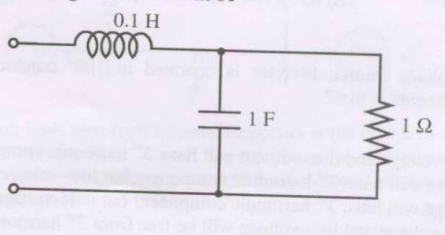
\includegraphics[width=\columnwidth]{Fig/q22.png}
    \caption{}
\end{figure}

\begin{multicols}{4}
\begin{enumerate}
    \item $1$ rad/s
    \item $2$ rad/s
    \item $3$ rad/s
    \item $4$ rad/s
\end{enumerate}
\end{multicols}
\hfill (GATE EE 2008)


\item Assuming ideal elements in the circuit shown below, the voltage $v_{ab}$ will be

\begin{figure}[H]
    \centering
    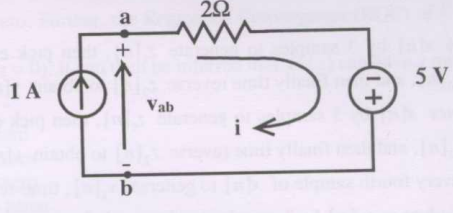
\includegraphics[width=\columnwidth]{Fig/q23.png}
    \caption{}
\end{figure}

\begin{multicols}{4}
\begin{enumerate}
    \item $-3$ V
    \item $0$ V
    \item $3$ V
    \item $5$ V
\end{enumerate}
\end{multicols}
\hfill (GATE EE 2008)




\item A capacitor consists of two metal plates each $500 \times 500$ mm$^{2}$ and spaced $6$ mm apart. The space between the metal plates is filled with a glass plate of $4$ mm thickness and a layer of paper of $2$ mm thickness. The relative permittivities of the glass and paper are $8$ and $2$ respectively. Neglecting the fringing effect, the capacitance will be (Given that $\varepsilon_0 = 8.85 \times 10^{-12}$ F/m)

\begin{multicols}{4}
\begin{enumerate}
    \item $983.33$ pF
    \item $1475$ pF
    \item $6637.5$ pF
    \item $9956.25$ pF
\end{enumerate}
\end{multicols}
\hfill (GATE EE 2008)

\item A coil of 300 turns is wound on a non-magnetic core having a mean circumference of 300 mm and a cross-sectional area of 300 mm$^{2}$. The inductance of the coil corresponding to a magnetizing current of 3A will be (Given that $\mu_0 = 4\pi \times 10^{-7}$ H/m)

\begin{multicols}{4}
\begin{enumerate}
    \item $37.68$ $\mu$H
    \item $113.04$ $\mu$H
    \item $37.68$ mH
    \item $113.04$ mH
\end{enumerate}
\end{multicols}
\hfill (GATE EE 2008)

\item In the circuit shown in the figure, the value of the current $i$ will be given by

\begin{figure}[H]
    \centering
    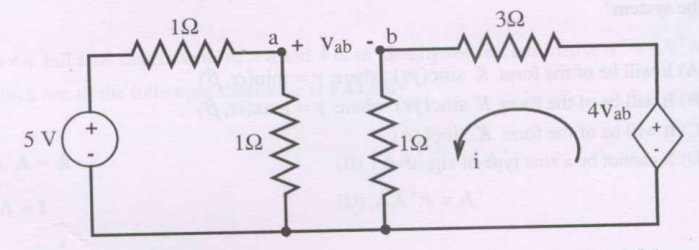
\includegraphics[width=\columnwidth]{Fig/q26.png}
    \caption{}
\end{figure}

\begin{multicols}{4}
\begin{enumerate}
    \item $0.31$ A
    \item $1.25$ A
    \item $1.75$ A
    \item $2.5$ A
\end{enumerate}
\end{multicols}
\hfill (GATE EE 2008)


\item Two point charges $Q_1 = 10$ $\mu$C and $Q_2 = 20$ $\mu$C are placed at coordinates $(1, 1, 0)$ and $(-1, -1, 0)$ respectively. The total electric flux passing through a plane $z = 20$ will be

\begin{multicols}{4}
\begin{enumerate}
    \item $7.5$ $\mu$C
    \item $13.5$ $\mu$C
    \item $15.0$ $\mu$C
    \item $22.5$ $\mu$C
\end{enumerate}
\end{multicols}
\hfill (GATE EE 2008)


\item Given a sequence $x[n]$, to generate the sequence $y[n]=x[3-4n]$, which one of the following procedures would be correct?

\begin{enumerate}
    \item First delay $x[n]$ by 3 samples to generate $z_{1}[n]$, then pick every $4^{\text{th}}$ sample of $z_{1}[n]$ to generate $z_{2}[n]$, and then finally time reverse $z_{2}[n]$ to obtain $y[n]$
    \item First advance $x[n]$ by 3 samples to generate $z_{1}[n]$, then pick every $4^{\text{th}}$ sample of $z_{1}[n]$ to generate $z_{2}[n]$, and then finally time reverse $z_{2}[n]$ to obtain $y[n]$
    \item First pick every fourth sample of $x[n]$ to generate $v_{1}[n]$, time-reverse $v_{1}[n]$ to obtain $v_{2}[n]$, and finally advance $v_{2}[n]$ by 3 samples to obtain $y[n]$
    \item First pick every fourth sample of $x[n]$ to generate $v_{1}[n]$, time-reverse $v_{1}[n]$ to obtain $v_{2}[n]$, and finally delay $v_{2}[n]$ by 3 samples to obtain $y[n]$
\end{enumerate}
\hfill (GATE EE 2008)


\item A system with input $x(t)$ and output $y(t)$ is defined by the input-output relation:
$$
y(t) = \int_{-\infty}^{-2t} x(\tau) \,d\tau
$$
The system will be

\begin{enumerate}
    \item causal, time-invariant and unstable
    \item causal, time-invariant and stable
    \item non-causal, time-invariant and unstable
    \item non-causal, time-variant and unstable
\end{enumerate}
\hfill (GATE EE 2008)


\item A signal $x(t)=\text{sinc}(\alpha t)$ where $\alpha$ is a real constant $\left(\text{sinc}(x) = \frac{\sin(\pi x)}{\pi x}\right)$ is the input to a Linear Time invariant system whose impulse response $h(t)=\text{sinc}(\beta t)$ where $\beta$ is a real constant. If $\min(\alpha, \beta)$ denotes the minimum of $\alpha$ and $\beta$, and similarly $\max(\alpha, \beta)$ denotes the maximum of $\alpha$ and $\beta$, and $K$ is a constant, which one of the following statements is true about the output of the system?

\begin{enumerate}
    \item It will be of the form $K \text{ sinc}(\gamma t)$ where $\gamma=\min(\alpha, \beta)$
    \item It will be of the form $K \text{ sinc}(\gamma t)$ where $\gamma=\max(\alpha, \beta)$
    \item It will be of the form $K \text{ sinc}(\alpha t)$
    \item It cannot be a sinc type of signal
\end{enumerate}
\hfill (GATE EE 2008)

\item Let $x(t)$ be a periodic signal with time period $T$. Let $y(t) = x(t-t_0)+x(t+t_0)$ for some $t_0$. The Fourier Series coefficients of $y(t)$ are denoted by $b_k$. If $b_k=0$ for all odd $k$, then $t_0$ can be equal to

\begin{multicols}{4}
\begin{enumerate}
    \item $T/8$
    \item $T/4$
    \item $T/2$
    \item $2T$
\end{enumerate}
\end{multicols}
\hfill (GATE EE 2008)


\item $H(z)$ is a transfer function of a real system. When a signal $x[n] = (1+j)^{n}$ is the input to such a system, the output is zero. Further, the Region Of Convergence (ROC) of $\left(1-\frac{1}{2}z^{-1}\right) H(z)$ is the entire Z-plane (except $z=0$). It can then be inferred that $H(z)$ can have a minimum of

\begin{enumerate}
    \item one pole and one zero
    \item one pole and two zeros
    \item two poles and one zero
    \item two poles and two zeros
\end{enumerate}
\hfill (GATE EE 2008)


\item Given $X(z)=\frac{z}{(z-a)^2}$ with $|z|>a$, the residue of $X(z)z^{n-1}$ at $z=a$ for $n \ge 0$ will be

\begin{multicols}{4}
\begin{enumerate}[label=(\Alph*)]
    \item $a^{n-1}$
    \item $a^{n}$
    \item $na^{n}$
    \item $na^{n-1}$
\end{enumerate}
\end{multicols}
\hfill (GATE EE 2008)


\item Consider function $f(x)=(x^2-4)^2$ where $x$ is a real number. Then the function has

\begin{enumerate}
    \item only one minimum
    \item only two minima
    \item three minima
    \item three maxima
\end{enumerate}
\hfill (GATE EE 2008)



\item Equation $e^x - 1 = 0$ is required to be solved using Newton's method with an initial guess $x_0 = -1$. Then, after one step of Newton's method, estimate $x_1$ of the solution will be given by

\begin{multicols}{4}
\begin{enumerate}
    \item $0.71828$
    \item $0.36784$
    \item $0.20587$
    \item $0.00000$
\end{enumerate}
\end{multicols}
\hfill (GATE EE 2008)

\item $A$ is a $m \times n$ full rank matrix with $m>n$ and $I$ is an identity matrix. Let matrix $A^{+}=(A^{\text{T}}A)^{-1}A^{\text{T}}$. Then, which one of the following statements is \textbf{FALSE}?

\begin{multicols}{2}
\begin{enumerate}
    \item $AA^{+}A = A$
    \item $(AA^{+})^2 = AA^{+}$
    \item $A^{+}A = I$
    \item $A A^{+}A = A^{+}$
\end{enumerate}
\end{multicols}
\hfill (GATE EE 2008)



\item A differential equation $\frac{dx}{dt} = e^{-2t}u(t)$ has to be solved using trapezoidal rule of integration with a step size $h=0.01$ s. Function $u(t)$ indicates a unit step function. If $x(0-) = 0$, then value of $x$ at $t=0.01$ s will be given by:

\begin{multicols}{4}
\begin{enumerate}
    \item $0.00099$
    \item $0.00495$
    \item $0.0099$
    \item $0.0198$
\end{enumerate}
\end{multicols}
\hfill (GATE EE 2008)

\item Let $P$ be a $2\times 2$ real orthogonal matrix and $\vec{x}$ is a real vector $[x_1, x_2]^T$ with length $\|\vec{x}\| = (x_1^2+x_2^2)^{1/2}$. Then, which one of the following statements is correct?

\begin{enumerate}
    \item $\|\vec{Px}\| \le \|\vec{x}\|$ where at least one vector satisfies $\|\vec{Px}\| < \|\vec{x}\|$
    \item $\|\vec{Px}\| = \|\vec{x}\|$ for all vectors $\vec{x}$
    \item $\|\vec{Px}\| \ge \|\vec{x}\|$ where at least one vector satisfies $\|\vec{Px}\| > \|\vec{x}\|$
    \item No relationship can be established between $\|\vec{x}\|$ and $\|\vec{Px}\|$
\end{enumerate}
\hfill (GATE EE 2008)


\item Let $x(t) = \text{rect}\left(t-\frac{1}{2}\right)$ (where $\text{rect}(x)=1$ for $-\frac{1}{2} \le x \le \frac{1}{2}$ and zero otherwise). Then if $\text{sinc}(x)=\frac{\sin(\pi x)}{\pi x}$, the Fourier Transform of $x(t)+x(-t)$ will be given by

\begin{multicols}{2}
\begin{enumerate}
    \item $\text{sinc}\left(\frac{\omega}{2\pi}\right)$
    \item $2 \text{ sinc}\left(\frac{\omega}{2\pi}\right)$
    \item $2 \text{ sinc}\left(\frac{\omega}{2\pi}\right)\cos\left(\frac{\omega}{2}\right)$
    \item $\text{sinc}\left(\frac{\omega}{2\pi}\right)\sin\left(\frac{\omega}{2}\right)$
\end{enumerate}
\end{multicols}
\hfill (GATE EE 2008)

\item Two perfectly matched silicon transistors are connected as shown in the figure. Assuming the $\beta$ of the transistors to be very high and the forward voltage drop in diodes to be $0.7$ V, the value of current I is

\begin{figure}[H]
    \centering
    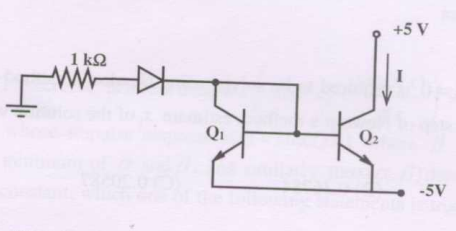
\includegraphics[width=\columnwidth]{Fig/q40.png}
    \caption{}
\end{figure}

\begin{multicols}{4}
\begin{enumerate}
    \item $0$ mA
    \item $3.6$ mA
    \item $4.3$ mA
    \item $5.7$ mA
\end{enumerate}
\end{multicols}


\item In the voltage doubler circuit shown in the figure, the switch 'S' is closed at t = 0. Assuming diodes $D_1$ and $D_2$ to be ideal, load resistance to be infinite and initial capacitor voltages to be zero, the steady state voltage across capacitors $C_1$ and $C_2$ will be

\begin{figure}[H]
    \centering
    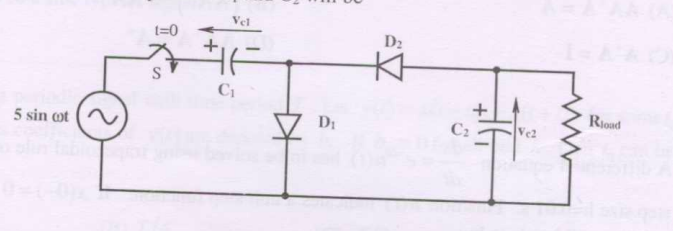
\includegraphics[width=\columnwidth]{Fig/q41.png}
    \caption{}
\end{figure}

\begin{multicols}{2}
\begin{enumerate}
    \item $v_{C1}=10$V, $v_{C2}=5$V
    \item $v_{C1}=10$V, $v_{C2}=-5$V
    \item $v_{C1}=5$V, $v_{C2}=10$V
    \item $v_{C1}=5$V, $v_{C2}=-10$V
\end{enumerate}
\end{multicols}
\hfill (GATE EE 2008)


\item  The block diagrams of two types of half wave rectifiers are shown in the figure. The transfer characteristics of the rectifiers are also shown within the block.
\begin{figure}[H]
    \centering
    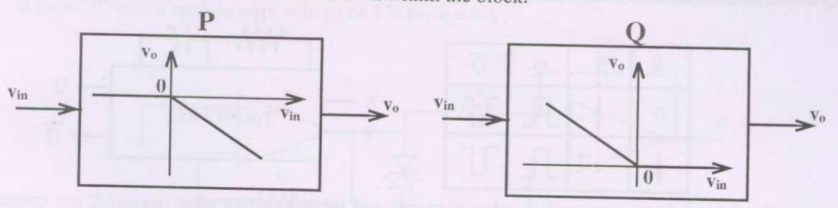
\includegraphics[width=\columnwidth]{Fig/q42.png}
    \caption{}
\end{figure}
\begin{enumerate}
\item 
\begin{figure}[H]
    \centering
    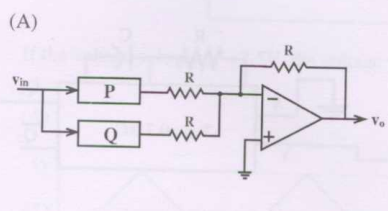
\includegraphics[width=\columnwidth]{Fig/q41-A.png}
    \caption{}
\end{figure}
\item \begin{figure}[H]
    \centering
    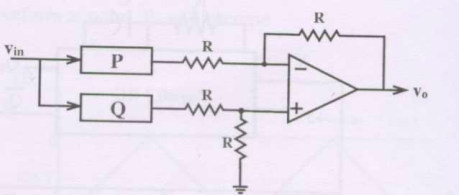
\includegraphics[width=\columnwidth]{Fig/q41-B.png}
    \caption{}
\end{figure}
\item \begin{figure}[H]
    \centering
    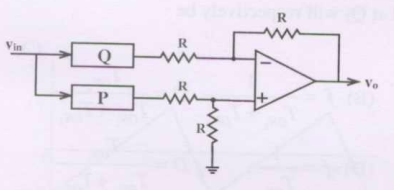
\includegraphics[width=\columnwidth]{Fig/q41-C.png}
    \caption{}
\end{figure}
\item 
\begin{figure}[H]
    \centering
    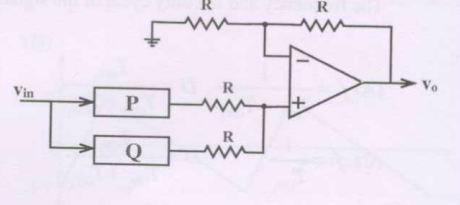
\includegraphics[width=\columnwidth]{Fig/q41-D.png}
    \caption{}
\end{figure}

\end{enumerate}
\hfill (GATE EE 2008)

\item A $3$ line to $8$ line decoder, with active low outputs, is used to implement a 3-variable Boolean function as shown in the figure.

\begin{figure}[H]
    \centering
    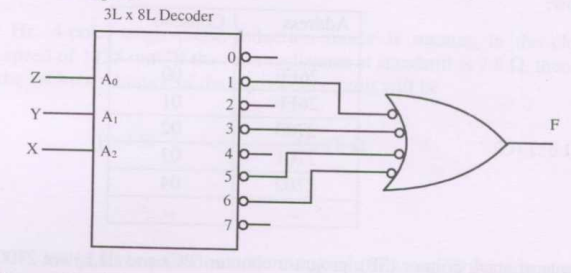
\includegraphics[width=\columnwidth]{Fig/q43.png}
\end{figure}

The simplified form of Boolean function $F(A,B,C)$ implemented in 'Product of Sum' form will be


\begin{enumerate}
    \item $(X+Z).(\bar{X}+\bar{Y}+\bar{Z}).(Y+Z)$
    \item $(B+\bar{Z}).(X+Y+Z).(\bar{Y}+\bar{Z})$
    \item $(\bar{X}+\bar{Y}+\bar{Z}).(\bar{X}+Y+Z).(X+\bar{Y}+Z).(X+Y+\bar{Z})$
    \item $(\bar{X}+\bar{Y}+\bar{Z}).(\bar{X}+Y+\bar{Z}).(X+Y+\bar{Z}).(X+\bar{Y}+\bar{Z})$
\end{enumerate}


\item  The truth table of a monoshot shown in the figure is given in the table below:
\begin{figure}[H]
    \centering
    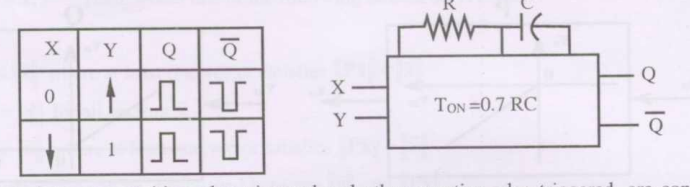
\includegraphics[width=\columnwidth]{Fig/q44.png}
    \caption{}
\end{figure}

Two monoshots, one positive edge triggered and other negative edge triggered, are connected as shown in the figure. The pulse widths of the two monoshot outputs, $Q_1$ and $Q_2$, are $T_{ON_1}$ and $T_{ON_2}$, respectively.

\begin{figure}[H]
    \centering
    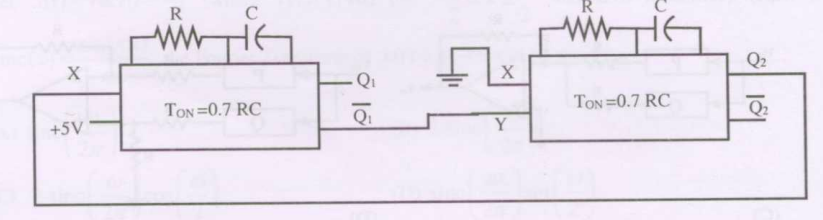
\includegraphics[width=\columnwidth]{Fig/q44-2.png}
    \caption{}
\end{figure}
The frequency and the duty cycle of the signal at $Q_1$ will respectively be

\begin{multicols}{2}
\begin{enumerate}
    \item $f = \frac{1}{T_{ON_1}+T_{ON_2}}, D = \frac{T_{ON_1}}{T_{ON_1}+T_{ON_2}}$
    \item $f = \frac{1}{T_{ON_1}+T_{ON_2}}, D = \frac{T_{ON_2}}{T_{ON_1}+T_{ON_2}}$
    \item $f = \frac{1}{T_{ON_1}}, D = \frac{T_{ON_1}}{T_{ON_1}+T_{ON_2}}$
    \item $f = \frac{1}{T_{ON_2}}, D = \frac{T_{ON_1}}{T_{ON_1}+T_{ON_2}}$
\end{enumerate}
\end{multicols}
\hfill (GATE EE 2008)

\item 
The contents (in Hexadecimal) of some of the memory locations in an 8085A based system are given below:

\begin{center}
\begin{tabular}{|c|c|}
\hline
Address & Contents \\
\hline
... & ... \\
\hline
26FE & 00 \\
\hline
26FF & 01 \\
\hline
2700 & 02 \\
\hline
2701 & 03 \\
\hline
2702 & 04 \\
\hline
... & ... \\
\hline
\end{tabular}
\end{center}

The contents of stack pointer (SP), program counter (PC) and (H,L) are 2700H, 2100H and 0000H respectively. When the following sequence of instructions are executed,
\vspace{0.5em}
\begin{verbatim}
2100 H: DAD SP
2101 H: PCHL
\end{verbatim}
\vspace{0.5em}
the contents of (SP) and (PC) at the end of execution will be

\begin{multicols}{2}
\begin{enumerate}
    \item (PC) = 2102H, (SP) = 2700H
    \item (PC) = 2700H, (SP) = 2700H
    \item (PC) = 2800H, (SP) = 26FEH
    \item (PC) = 2A02H, (SP) = 2702H
\end{enumerate}
\end{multicols}
\hfill (GATE EE 2008)


\item  A
at waveform point 'P' with generator circuit using OPAMPs is shown in the figure. It produces a triangular wave a peak to peak voltage of 5 V for v; = 0 V

\begin{center}
    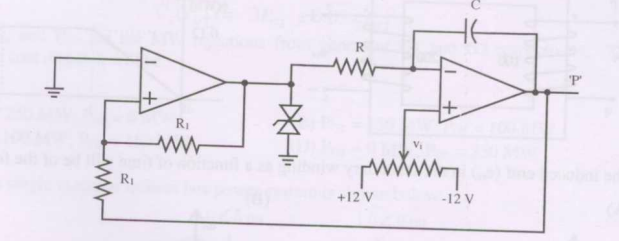
\includegraphics[width=\columnwidth]{Fig/q46.png}
    \caption{}
\end{center}
If the voltage v; is made +2.5V, the voltage waveform at point 'P' will become
\begin{enumerate}
        
    \item 
    \begin{figure}[H]
        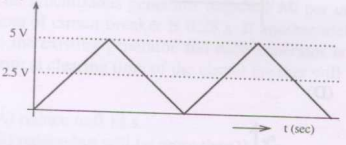
\includegraphics[width=\columnwidth]{Fig/q46-A.png}
        \caption{}
    \end{figure}


    \item 
    \begin{figure}[H]
        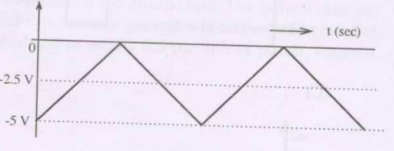
\includegraphics[width=\columnwidth]{Fig/q46-B.png}
        \caption{}
    \end{figure}

    
    \item 
    \begin{figure}[H]
        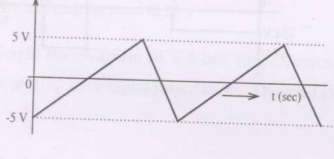
\includegraphics[width=\columnwidth]{Fig/q46-C.png}
        \caption{}
    \end{figure}


    \item 
    \begin{figure}[H]
        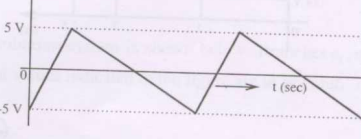
\includegraphics[width=\columnwidth]{Fig/q46-D.png}
        \caption{}
    \end{figure}




\end{enumerate}
\hfill (GATE EE 2008) \\[5mm]



\item A $230$V, $50$ Hz, $4$-pole, single-phase induction motor is rotating in the clockwise (forward) direction at a speed of $1425$ rpm. If the rotor resistance at standstill is $7.8 \Omega$, then the effective rotor resistance in the backward branch of the equivalent circuit will be

\begin{multicols}{4}
\begin{enumerate}
    \item $2 \Omega$
    \item $4 \Omega$
    \item $78 \Omega$
    \item $156 \Omega$
\end{enumerate}
\end{multicols}
\hfill (GATE EE 2008)


\item A $400$ V, $50$ Hz, $30$ hp, three-phase induction motor is drawing $50$ A current at $0.8$ power factor lagging. The stator and rotor copper losses are $1.5$ kW and $900$ W respectively. The friction and windage losses are $1050$ W and the core losses are $1200$ W. The air-gap power of the motor will be

\begin{multicols}{4}
\begin{enumerate}
    \item $23.06$ kW
    \item $24.11$ kW
    \item $25.01$ kW
    \item $26.21$ kW
\end{enumerate}
\end{multicols}
\hfill (GATE EE 2008)



\item The core of a two-winding transformer is subjected to a magnetic flux variation as indicated in the figure

\begin{figure}[H]
    \centering
    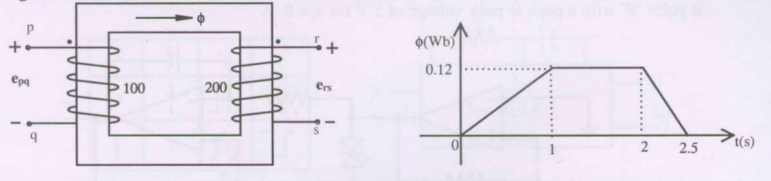
\includegraphics[width=\columnwidth]{Fig/q49.png}
    \caption{}
\end{figure}
The induced emf $e_(rs)$ in the secondary winding as a function of time will be of the form
\begin{enumerate}
        
    \item 
    \begin{figure}[H]
        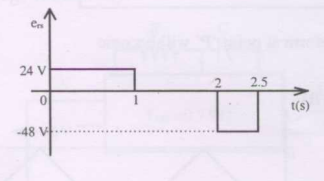
\includegraphics[width=\columnwidth]{Fig/q49-A.png}
        \caption{}
    \end{figure}


    \item 
    \begin{figure}[H]
        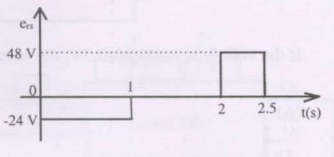
\includegraphics[width=\columnwidth]{Fig/q49-B.png}
        \caption{}
    \end{figure}

    
    \item 
    \begin{figure}[H]
        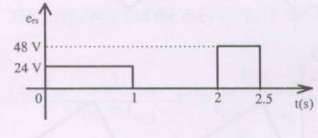
\includegraphics[width=\columnwidth]{Fig/q49-C.png}
        \caption{}
    \end{figure}


    \item 
    \begin{figure}[H]
        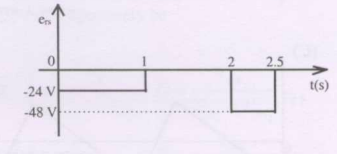
\includegraphics[width=\columnwidth]{Fig/q49-D.png}\caption{}
    \end{figure}




\end{enumerate}
\hfill (GATE EE 2008) \\[5mm]





\item Voltage phasors at the two terminals of a transmission line of length $70$ km have a magnitude of $1.0$ per unit but are $180$ degrees out of phase. Assuming that the maximum load current in the line is $1/5^{\text{th}}$ of minimum 3-phase fault current, which one of the following transmission line protection schemes will NOT pick up for this condition?

\begin{enumerate}
    \item Distance protection using mho relays with zone-$1$ set to $80\%$ of the line impedance
    \item Directional overcurrent protection set to pick up at $1.25$ times the maximum load current
    \item Pilot relaying system with directional comparison scheme
    \item Pilot relaying system with segregated phase comparison scheme
\end{enumerate}
\hfill (GATE EE 2008)



\item A lossless transmission line having Surge Impedance Loading (SIL) of $2280$ MW is provided with a uniformly distributed series capacitive compensation of $30 \%$. Then, SIL of the compensated transmission line will be

\begin{enumerate}
    \item $1835$ MW
    \item $2280$ MW
    \item $2725$ MW
    \item $3257$ MW
\end{enumerate}
\hfill (GATE EE 2008)


\item A lossless power system has to serve a load of $250$ MW. There are two generators ($G_1$ and $G_2$) in the system with cost curves $C_1$ and $C_2$ respectively defined as follows:
\begin{center}
$
C_1(P_{G1}) = P_{G1}+0.055 \times P_{G1}^2
$\\
$
C_2(P_{G2}) = 3P_{G2}+0.03 \times P_{G2}^2
$\\
\end{center}
where $P_{G1}$ and $P_{G2}$ are the MW injections from generator $G_1$ and $G_2$ respectively. Then, the minimum cost dispatch will be

\begin{multicols}{2}
\begin{enumerate}
    \item $P_{G1} = 250$ MW; $P_{G2} = 0$ MW
    \item $P_{G1} = 150$ MW; $P_{G2} = 100$ MW
    \item $P_{G1} = 100$ MW; $P_{G2} = 150$ MW
    \item $P_{G1} = 0$ MW; $P_{G2} = 250$ MW
\end{enumerate}
\end{multicols}
\hfill (GATE EE 2008)


\item A lossless single machine infinite bus power system is shown below:

\begin{figure}[H]
    \centering
    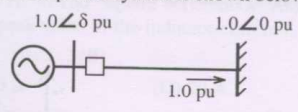
\includegraphics[width=\columnwidth]{Fig/q53.png}
    \caption{}
\end{figure}

The synchronous generator transfers $1.0$ per unit of power to the infinite bus. The critical clearing time of circuit breaker is $0.28$ s. If another identical synchronous generator is connected in parallel to the existing generator and each generator is scheduled to supply $0.5$ per unit of power, then the critical clearing time of the circuit breaker will

\begin{enumerate}
    \item reduce to $0.14$ s
    \item reduce but will be more than $0.14$ s
    \item remain constant at $0.28$ s
    \item increase beyond $0.28$ s
\end{enumerate}
\hfill (GATE EE 2008)


\item Single line diagram of a 4-bus single source distribution system is shown below. Branches $e_1$, $e_2$, $e_3$ and $e_4$ have equal impedances. The load current values indicated in the figure are in per unit.

\begin{figure}[H]
    \centering
    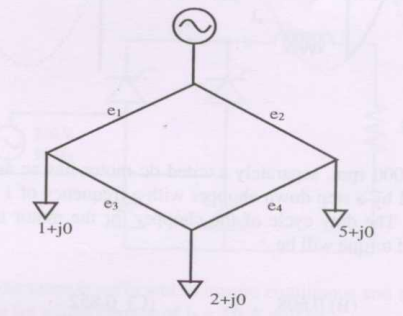
\includegraphics[width=\columnwidth]{Fig/q54.png}
\end{figure}

Distribution company's policy requires radial system operation with minimum loss. This can be achieved by opening of the branch

\begin{multicols}{4}
\begin{enumerate}
    \item $e_1$
    \item $e_2$
    \item $e_3$
    \item $e_4$
\end{enumerate}
\end{multicols}
\hfill (GATE EE 2008)



\item A single phase fully controlled bridge converter supplies a load drawing constant and ripple free load current. If the triggering angle is $30\degree$, the input power factor will be

\begin{multicols}{4}
\begin{enumerate}
    \item $0.65$
    \item $0.78$
    \item $0.85$
    \item $0.866$
\end{enumerate}
\end{multicols}
\hfill (GATE EE 2008)


\item A single-phase half controlled converter shown in the figure is feeding power to highly inductive
load. The converter is operating at a firing angle of $60\degree$
\begin{center}
    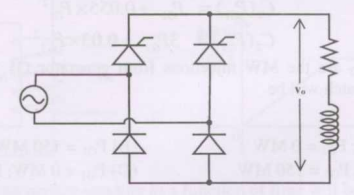
\includegraphics[width=\columnwidth]{Fig/q56.png}
    \caption{}
\end{center}
If the firing pulses are suddenly removed, the steady state voltage $v_o$ waveform of the converter
will become
\begin{enumerate}
        
    \item 
    \begin{figure}[H]
        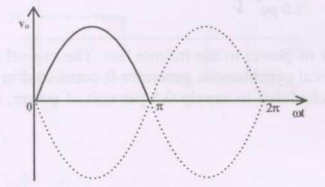
\includegraphics[width=\columnwidth]{Fig/q56-A.png}\caption{}
    \end{figure}


    \item 
    \begin{figure}[H]
        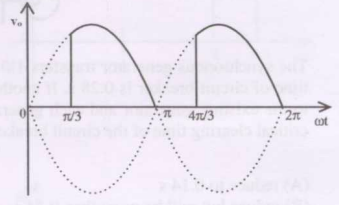
\includegraphics[width=\columnwidth]{Fig/q56-B.png}\caption{}
    \end{figure}

    
    \item 
    \begin{figure}[H]
        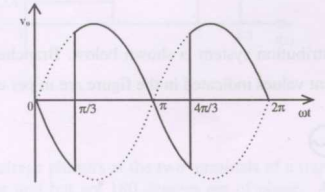
\includegraphics[width=\columnwidth]{Fig/q56-C.png}\caption{}
    \end{figure}


    \item 
    \begin{figure}[H]
        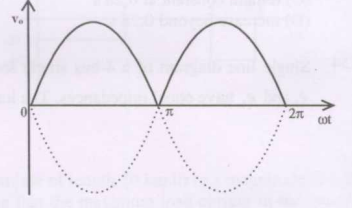
\includegraphics[width=\columnwidth]{Fig/q56-D.png}\caption{}
    \end{figure}




\end{enumerate}
\hfill (GATE EE 2008) \\[5mm]







\item A $220$ V, $20$ A, $1000$ rpm, separately excited dc motor has an armature resistance of $2.5 \Omega$. The motor is controlled by a step down chopper with a frequency of $1$ kHz. The input dc voltage to the chopper is $250$ V. The duty cycle of the chopper for the motor to operate at a speed of $600$ rpm delivering the rated torque will be

\begin{multicols}{4}
\begin{enumerate}
    \item $0.518$
    \item $0.608$
    \item $0.852$
    \item $0.902$
\end{enumerate}
\end{multicols}
\hfill (GATE EE 2008)

\item A $220$ V, $1400$ rpm, $40$ A separately excited dc motor has an armature resistance of $0.4 \Omega$. The motor is fed from a single phase circulating current dual converter with an input ac line voltage of $220$ V (rms). The approximate firing angles of the dual converter for motoring operation at $50\%$ of rated torque and $1000$ rpm will be

\begin{multicols}{4}
\begin{enumerate}
    \item $43\degree, 137\degree$
    \item $43\degree, 47\degree$
    \item $39\degree, 141\degree$
    \item $39\degree, 51\degree$
\end{enumerate}
\end{multicols}
\hfill (GATE EE 2008)


\item A single phase voltage source inverter is feeding a purely inductive load as shown in the figure.

\begin{figure}[H]
    \centering
    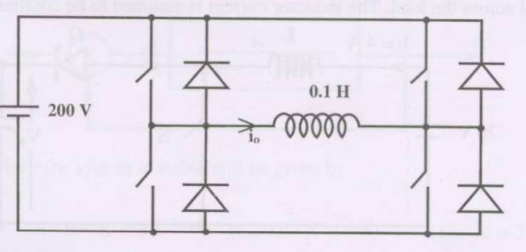
\includegraphics[width=\columnwidth]{Fig/q59.png}
    \caption{}
\end{figure}

The inverter is operated at 50 Hz in $180\degree$ square wave mode. Assume that the load current does not have any dc component. The peak value of the inductor current $i_o$ will be

\begin{multicols}{4}
\begin{enumerate}
    \item $6.37$ A
    \item $10$ A
    \item $20$ A
    \item $40$ A
\end{enumerate}
\end{multicols}
\hfill (GATE EE 2008)


\item A $400$ V, $50$ Hz, $4$ pole, $1400$ rpm, star connected squirrel cage induction motor has the following parameters referred to the stator:
$$
R_s = 1.0 \Omega, X_s = X_r' = 1.5 \Omega
$$
Neglect stator resistance and core and rotational losses of the motor.
The motor is controlled from a 3-phase voltage source inverter with constant V/f control. The stator line-to-line voltage (rms) and frequency to obtain the maximum torque at starting will be:

\begin{multicols}{4}
\begin{enumerate}
    \item $20.6$ V, $2.7$ Hz
    \item $133.3$ V, $16.7$ Hz
    \item $266.6$ V, $33.3$ Hz
    \item $323.3$ V, $40.3$ Hz
\end{enumerate}
\end{multicols}
\hfill (GATE EE 2008)



\item A single phase fully controlled converter bridge is used for electrical braking of a separately excited dc motor. The dc motor load is represented by an equivalent circuit as shown in the figure.

\begin{figure}[H]
    \centering
    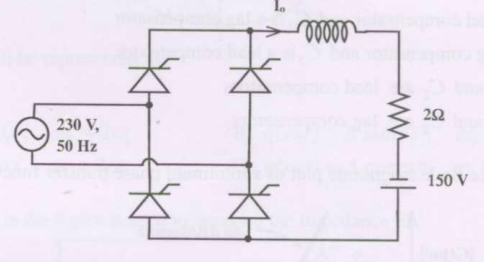
\includegraphics[width=\columnwidth]{Fig/q61.png}
    \caption{}
\end{figure}

Assume that the load inductance is sufficient to ensure continuous and ripple free load current. The firing angle of the bridge for a load current of $I_o = 10$ A will be

\begin{multicols}{4}
\begin{enumerate}
    \item $44\degree$
    \item $51\degree$
    \item $129\degree$
    \item $136\degree$
\end{enumerate}
\end{multicols}
\hfill (GATE EE 2008)



\item A three phase fully controlled bridge converter is feeding a load drawing a constant and ripple free load current of 10 A at a firing angle of $30\degree$. The approximate Total Harmonic Distortion (\%THD) and the rms value of fundamental component of the input current will respectively be

\begin{multicols}{4}
\begin{enumerate}
    \item $31\%$ and $6.8$ A
    \item $31\%$ and $7.8$ A
    \item $66\%$ and $6.8$ A
    \item $66\%$ and $7.8$ A
\end{enumerate}
\end{multicols}
\hfill (GATE EE 2008)


\item In the circuit shown in the figure, the switch is operated at a duty cycle of $0.5$. A large capacitor is connected across the load. The inductor current is assumed to be continuous.

\begin{figure}[H]
    \centering
    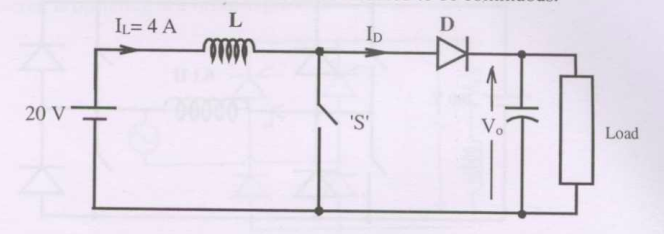
\includegraphics[width=\columnwidth]{Fig/q64.png}
    \caption{}
\end{figure}

The average voltage across the load and the average current through the diode will respectively be

\begin{multicols}{4}
\begin{enumerate}
    \item $10$ V, $2$ A
    \item $10$ V, $8$ A
    \item $40$ V, $2$ A
    \item $40$ V, $8$ A
\end{enumerate}
\end{multicols}
\hfill (GATE EE 2008)


\item The transfer function of a linear time invariant system is given as
$$
G(s)=\frac{1}{s^2+3s+2}
$$
The steady state value of the output of this system for a unit impulse input applied at time instant $t=1$ will be

\begin{multicols}{4}
\begin{enumerate}
    \item $0$
    \item $0.5$
    \item $1$
    \item $2$
\end{enumerate}
\end{multicols}
\hfill (GATE EE 2008)


\item The transfer functions of two compensators are given below:
$$
C_1 = \frac{10(s+1)}{(s+10)}, \quad C_2 = \frac{s+10}{10(s+1)}
$$

Which one of the following statements is correct?
\begin{enumerate}
    \item $C_1$ is a lead compensator and $C_2$ is a lag compensator
    \item $C_1$ is a lag compensator and $C_2$ is a lead compensator
    \item Both $C_1$ and $C_2$ are lead compensators
    \item Both $C_1$ and $C_2$ are lag compensators
\end{enumerate}
\hfill (GATE EE 2008)


\item The asymptotic Bode magnitude plot of a minimum phase transfer function is shown in the figure:

\begin{figure}[H]
    \centering
    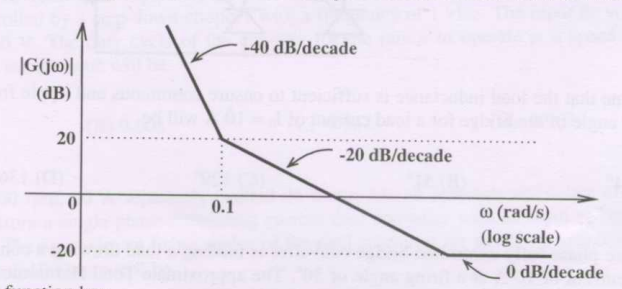
\includegraphics[width=\columnwidth]{Fig/q66.png}
    \caption{}
\end{figure}

This transfer function has

\begin{multicols}{2}
\begin{enumerate}
    \item Three poles and one zero
    \item Two poles and one zero
    \item Two poles and two zeros
    \item One pole and two zeros
\end{enumerate}
\end{multicols}
\hfill (GATE EE 2008)


\item Figure shows a feedback system where $K>0$.

\begin{figure}[H]
    \centering
    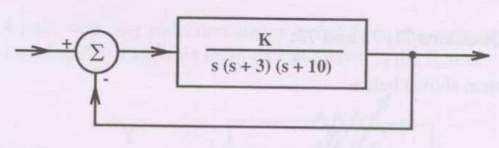
\includegraphics[width=\columnwidth]{Fig/q67.png}
    \caption{}
\end{figure}

The range of $K$ for which the system is stable will be given by

\begin{multicols}{4}
\begin{enumerate}
    \item $0 < K < 30$
    \item $0 < K < 39$
    \item $0 < K < 390$
    \item $K > 390$
\end{enumerate}
\end{multicols}
\hfill (GATE EE 2008)



\item The transfer function of a system is given as
$$
\frac{100}{s^2+20s+100}
$$
This system is

\begin{multicols}{2}
\begin{enumerate}
    \item an overdamped system
    \item an underdamped system
    \item a critically damped system
    \item an unstable system
\end{enumerate}
\end{multicols}
\hfill (GATE EE 2008)




\item Two sinusoidal signals $p(\omega_1 t) = A \sin \omega_1 t$ and $q(\omega_2 t)$ are applied to X and Y inputs of a dual channel CRO. The Lissajous figure displayed on the screen is shown below:

\begin{figure}[H]
    \centering
    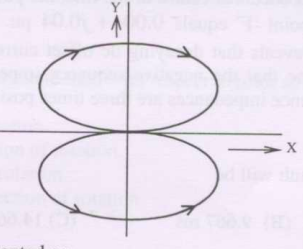
\includegraphics[width=\columnwidth]{Fig/q69.png}
    \caption{}
\end{figure}

The signal $q(\omega_2 t)$ will be represented as

\begin{multicols}{2}
\begin{enumerate}
    \item $q(\omega_2 t) = A \sin \omega_2 t, \quad \omega_2 = 2\omega_1$
    \item $q(\omega_2 t) = A \sin \omega_2 t, \quad \omega_2 = \omega_1/2$
    \item $q(\omega_2 t) = A \cos \omega_2 t, \quad \omega_2 = 2\omega_1$
    \item $q(\omega_2 t) = A \cos \omega_2 t, \quad \omega_2 = \omega_1/2$
\end{enumerate}
\end{multicols}
\hfill (GATE EE 2008)



\item The ac bridge shown in the figure is used to measure the impedance Z.

\begin{figure}[H]
    \centering
    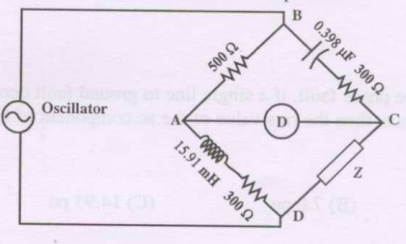
\includegraphics[width=\columnwidth]{Fig/q70.png}
    \caption{}
\end{figure}

If the bridge is balanced for oscillator frequency $f=2$ kHz, then the impedance Z will be

\begin{multicols}{4}
\begin{enumerate}
    \item $(260 + j0)\,\Omega$
    \item $(0 + j200)\,\Omega$
    \item $(260 - j200)\,\Omega$
    \item $(260 + j200)\,\Omega$
\end{enumerate}
\end{multicols}
\hfill (GATE EE 2008)


\begin{center}
\textbf{Common Data Questions}
\end{center}

\textbf{Common Data for Questions 71, 72 and 73:}

Consider a power system shown below:

\begin{figure}[H]
    \centering
    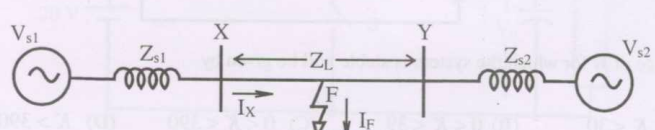
\includegraphics[width=\columnwidth]{Fig/comp1.png}
    \caption{}
\end{figure}

Given that:
$V_{s1} = V_{s2} = 1.0+j0.0$ pu;
The positive sequence impedances are $Z_{s1} = Z_{s2} = 0.001+j0.01$ pu and $Z_L = 0.006+j0.06$ pu.

3-phase Base MVA = 100

Voltage base = 400 kV (Line to Line)

Nominal system frequency = 50 Hz

The reference voltage for phase 'a' is defined as $v(t) = V_m \cos(\omega t)$.

A symmetrical three phase fault occurs at centre of the line, i.e. point 'F' at time $t_o$. The positive sequence impedance from source $S_1$ to point 'F' equals $0.004+j0.04$ pu. The waveform corresponding to phase 'a' fault current from bus X reveals that decaying dc offset current is negative and in magnitude at its maximum initial value. Assume that the negative sequence impedances are equal to positive sequence impedances, and the zero sequence impedances are three times positive sequence impedances. \\[10mm]


\item The instant $(t_0)$ of the fault will be

\begin{multicols}{2}
\begin{enumerate}
    \item 4.682 ms
    \item 9.667 ms
    \item 14.667 ms
    \item 19.667 ms
\end{enumerate}
\end{multicols}
\hfill (GATE EE 2008) \\[5mm]

\item  The rms value of the ac component of fault current ($I_x$) will be
\begin{enumerate}
\begin{multicols}{4}
    \item 3.59 kA
    \item 5.07 kA
    \item 7.18 kA
    \item 10.15 kA
    \end{multicols}
\end{enumerate}
\hfill (GATE EE 2008) \\[5mm]

\item Instead of the three phase fault, if a single line to ground fault occurs on phase `a' at point `F' with zero fault impedance, then the rms value of the ac component of fault current ($I_x$) for phase `a' will be
\begin{multicols}{4}
\begin{enumerate}
    \item 4.97 pu
    \item 7.0 pu
    \item 14.93 pu
    \item 29.85 pu
\end{enumerate}
\end{multicols}
\hfill (GATE EE 2008) \\[5mm]



\textbf{Common Data for Questions 74 and 75:}

A 3-phase, 440 V, 50 Hz, 4-pole, slip ring induction motor is fed from the rotor side through an auto-transformer and the stator is connected to a variable resistance as shown in the figure.

\begin{figure}[H]
    \centering
    \includegraphics[width=\columnwidth]{Fig/comp2.png}
    \caption{}
    
\end{figure}


The motor is coupled to a 220 V, separately excited, dc generator feeding power to a fixed resistance of 10 $\Omega$. Two-wattmeter method is used to measure the input power to induction motor. The variable resistance is adjusted such that the motor runs at 1410 rpm and the following readings were recorded:  


$W_1 = 1800~\text{W}, \quad W_2 = -200~\text{W}$  \\[5mm]


\item The speed of rotation of stator magnetic field with respect to rotor structure will be

\begin{enumerate}
    \item 90 rpm in the direction of rotation.
    \item 90 rpm in the opposite direction of rotation.
    \item 1500 rpm in the direction of rotation.
    \item 1500 rpm in the opposite direction of rotation.
\end{enumerate}

\hfill (GATE EE 2008) \\[5mm]

\item eglecting all losses of both the machines, the dc generator power output and the current through resistance ($R_{ex}$) will respectively be
\begin{multicols}{2}
\begin{enumerate}
    \item 96 W, 3.10 A
    \item 120 W, 3.46 A
    \item 1504 W, 12.26 A
    \item 1880 W, 13.71 A
\end{enumerate}
\end{multicols}


\begin{center}
\textbf{Linked Answer Questions: Q.76 to Q.85 carry two marks each.}
\end{center}

\textbf{Statement for Linked Answer Questions 76 and 77:}\\

The current $i(t)$ sketched in the figure flows through an initially uncharged $0.3~\text{nF}$ capacitor.

\begin{center}
\includegraphics[width=\columnwidth]{Fig/comp3.png}
\caption{}
\end{center}

\item  The charge stored in the capacitor at $t = 5~\mu\text{s}$ will be
\begin{multicols}{4}
\begin{enumerate}
    \item 8 nC
    \item 10 nC
    \item 13 nC
    \item 16 nC
\end{enumerate}
\end{multicols}
\hfill (GATE EE 2008) \\[5mm]

\item The capacitor charged up to $5~\mu\text{s}$, as per the current profile given in the figure, is connected across an inductor of $0.6~\text{mH}$. Then the value of voltage across the capacitor after $1~\mu\text{s}$ will approximately be
\begin{multicols}{4}
\begin{enumerate}
    \item 18.8 V
    \item 23.5 V
    \item $-23.5$ V
    \item $-30.6$ V
\end{enumerate}
\end{multicols}
\hfill (GATE EE 2008) \\[5mm]

\textbf{Statement for Linked Answer Questions 78 and 79:}\\

The state space equation of a system is described by
\begin{center}
\textbf{x = Ax + Bu}\\
\textbf{y = Cx}\\
\end{center}
where $x$ is state vector, $u$ is input, $y$ is output and
\[
A=\begin{bmatrix}0&1\\[2pt]0&-2\end{bmatrix},\qquad
B=\begin{bmatrix}0\\[2pt]1\end{bmatrix},\qquad
C=\begin{bmatrix}1&0\end{bmatrix}.
\]

\item The transfer function $G(s)$ of this system will be
\begin{multicols}{4}
\begin{enumerate}
    \item $\dfrac{s}{(s+2)}$
    \item $\dfrac{s+1}{s(s-2)}$
    \item $\dfrac{s}{(s-2)}$
    \item $\dfrac{1}{s(s+2)}$
\end{enumerate}
\end{multicols}
\hfill (GATE EE 2008) \\[5mm]


\item A unity feedback is provided to the above system $G(s)$ to make it a closed-loop system as shown.
\begin{figure}
    \centering
    \includegraphics[width=\columnwidth]{Fig/q79.png}
    \caption{}
\end{figure}

  For a unit step input $r(t)$, the steady state error in the output will be
\begin{multicols}{4}
\begin{enumerate}
    \item 0
    \item 1
    \item 2
    \item $\infty$
\end{enumerate}
\end{multicols}
\hfill (GATE EE 2008) \\[5mm]


\textbf{Statement for Linked Answer Questions 80 and 81:}\\

A general filter circuit is shown in the figure:

\begin{figure}
    \centering
    \includegraphics[width=\columnwidth]{Fig/comp4.png}
    \caption{}
\end{figure}

\item  If $R_1 = R_2 = R_A$ and $R_3 = R_4 = R_B$, the circuit acts as a
\begin{multicols}{2}
\begin{enumerate}
    \item all pass filter
    \item band pass filter
    \item high pass filter
    \item low pass filter
\end{enumerate}
\end{multicols}
\hfill (GATE EE 2008) \\[5mm]

\item  The output of the filter in Q.80 is given to the circuit shown in figure:

\begin{figure}
    \centering
    \includegraphics[width=\columnwidth]{Fig/q81.png}
    \caption{}
\end{figure}
The gain vs frequency characteristic of the output ($v_o$) will be
\begin{enumerate}
        
    \item 
    \begin{figure}[H]
        \includegraphics[width=\columnwidth]{Fig/q81-A.png}
        \caption{}
    \end{figure}


    \item 
    \begin{figure}[H]
        \includegraphics[width=\columnwidth]{Fig/q81-B.png}\caption{}
    \end{figure}

    
    \item 
    \begin{figure}[H]
        \includegraphics[width=\columnwidth]{Fig/q81-C.png}
        \caption{}
    \end{figure}


    \item 
    \begin{figure}[H]
        \includegraphics[width=\columnwidth]{Fig/q81-D.png}\caption{}
    \end{figure}




\end{enumerate}
\hfill (GATE EE 2008) \\[5mm]


\textbf{Statement for Linked Answer Questions 82 and 83:}\\

\item A $240\ \text{V}$, dc shunt motor draws $15\ \text{A}$ while supplying the rated load at a speed of $80\ \text{rad/s}$. The armature resistance is $0.5\ \Omega$ and the field winding resistance is $80\ \Omega$.
\\ [5mm]

\item The net voltage across the armature resistance at the time of plugging will be

\begin{multicols}{2}
\begin{enumerate}
    \item 6 V
    \item 234 V
    \item 240 V
    \item 474 V
\end{enumerate}
\end{multicols}
\hfill (GATE EE 2008) \\[5mm]

\item The external resistance to be added in the armature circuit to limit the armature current to $125\%$ of its rated value is

\begin{multicols}{2}
\begin{enumerate}
    \item 31.1 $\Omega$
    \item 31.9 $\Omega$
    \item 15.1 $\Omega$
    \item 15.9 $\Omega$
\end{enumerate}
\end{multicols}
\hfill (GATE EE 2008) \\[5mm]

\textbf{Statement for Linked Answer Questions 84 and 85:}\\

 A synchronous motor is connected to an infinite bus at $1.0\ \text{pu}$ voltage and draws $0.6\ \text{pu}$ current at unity power factor. Its synchronous reactance is $1.0\ \text{pu}$ and resistance is negligible\\

\item  Keeping the excitation voltage same, the load on the motor is increased such that the motor current increases by $20\%$. The operating power factor will become

\begin{multicols}{2}
\begin{enumerate}
  \item $0.995$ lagging
  \item $0.995$ leading
  \item $0.791$ lagging
  \item $0.848$ leading
\end{enumerate}
\end{multicols}
\hfill (GATE EE 2008) \\[5mm]





\end{enumerate}
    
\end{document}
